%\title{LaTeX Portrait Poster Template}
%%%%%%%%%%%%%%%%%%%%%%%%%%%%%%%%%%%%%%%%%
% a0poster Portrait Poster
% LaTeX Template
% Version 1.0 (22/06/13)
%
% The a0poster class was created by:
% Gerlinde Kettl and Matthias Weiser (tex@kettl.de)
% 
% This template has been downloaded from:
% http://www.LaTeXTemplates.com
%
% License:
% CC BY-NC-SA 3.0 (http://creativecommons.org/licenses/by-nc-sa/3.0/)
%
%%%%%%%%%%%%%%%%%%%%%%%%%%%%%%%%%%%%%%%%%

%----------------------------------------------------------------------------------------
%	PACKAGES AND OTHER DOCUMENT CONFIGURATIONS
%----------------------------------------------------------------------------------------

\documentclass[a0,portrait]{a0poster}

\usepackage{multicol} % This is so we can have multiple columns of text side-by-side
\columnsep=100pt % This is the amount of white space between the columns in the poster
\columnseprule=3pt % This is the thickness of the black line between the columns in the poster

\usepackage[svgnames]{xcolor} % Specify colors by their 'svgnames', for a full list of all colors available see here: http://www.latextemplates.com/svgnames-colors

\usepackage{times} % Use the times font
%\usepackage{palatino} % Uncomment to use the Palatino font

\usepackage{graphicx} % Required for including images
\graphicspath{{figures/}} % Location of the graphics files
\usepackage{booktabs} % Top and bottom rules for table
\usepackage[font=small,labelfont=bf]{caption} % Required for specifying captions to tables and figures
\usepackage{amsfonts, amsmath, amsthm, amssymb} % For math fonts, symbols and environments
\usepackage{wrapfig} % Allows wrapping text around tables and figures

\begin{document}

%----------------------------------------------------------------------------------------
%	POSTER HEADER 
%----------------------------------------------------------------------------------------

% The header is divided into two boxes:
% The first is 75% wide and houses the title, subtitle, names, university/organization and contact information
% The second is 25% wide and houses a logo for your university/organization or a photo of you
% The widths of these boxes can be easily edited to accommodate your content as you see fit

\begin{minipage}[b]{0.75\linewidth}
\VeryHuge \color{NavyBlue} \textbf{Geothermal Resources in Algeria} \color{Black}\\ % Title
\Huge\textit{Country Update}\\[2.4cm] % Subtitle
\huge \textbf{Hakim SAIBI}\\[0.5cm] % Author(s)
\huge Kyushu University, Department of Earth Resources Engineering, Japan\\[0.4cm] % University/organization
\Large \texttt{saibi-hakim@mine.kyushu-u.ac.jp} --- +81 (092) 802 3316\\
\end{minipage}
%
\begin{minipage}[b]{0.25\linewidth}

\includegraphics[width=7cm]{logo.png}\ 

\includegraphics[width=14cm]{logo-WGC.png}\\
\end{minipage}

\vspace{1cm} % A bit of extra whitespace between the header and poster content

%----------------------------------------------------------------------------------------

\begin{multicols}{3} % This is how many columns your poster will be broken into, a portrait poster is generally split into 2 columns

%----------------------------------------------------------------------------------------
%	ABSTRACT
%----------------------------------------------------------------------------------------

\color{Navy} % Navy color for the abstract

\begin{abstract}
The electrical energy from renewables in Algeria contributed about 3.4\% (280 MW) in 2008 of a total power of 8.1 GWe and will reach 5\% by the year 2017 according to the Algerian Electricity and Gas Regulation Commission (CREG). The country’s target is reaching 40\% by 2030. The geothermal resources in Algeria are of low-enthalpy type. Most of these geothermal resources are located in the north of the country and generate a heat discharge of 240 MWt.
\end{abstract}
%----------------------------------------------------------------------------------------
%	INTRODUCTION
%----------------------------------------------------------------------------------------

\color{Black} % SaddleBrown color for the introduction
\section*{Introduction}
Algeria is situated in northern Africa, bordering the Mediterranean Sea, between Morocco and Tunisia. Algeria has the 9th-largest reserves of natural gas in the world. It ranks 16th in proved oil reserves. Currently, more than 98 \% of Algeria's electricity generation comes from fossil-fuel resources. 
\begin{itemize}
\item Geothermal exploration program started in 1967 by National Oil Comapny SONATRACH.
\item From 1983 onwards the geothermal research has been continued by the Renewable Energies Center of Algeria (CDER).
\end{itemize}
%----------------------------------------------------------------------------------------
%	GEOLOGY
%----------------------------------------------------------------------------------------

\color{Black} % DarkSlateGray color for the rest of the content

\section*{Geology}
The geology of Algeria (Figure 1) is divided into two main structural units: the folded Tellian Domain in the North, and the Saharian Platform in the South, separated by the South Atlasic Flexure (Fabre, 1976). 
\begin{center}\vspace{1cm}
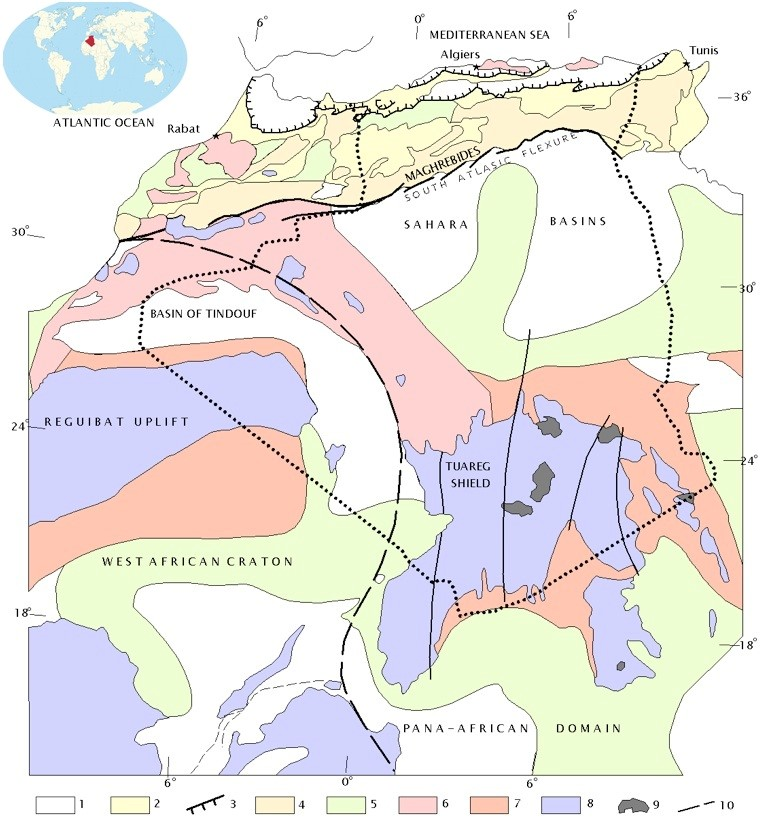
\includegraphics[width=0.8\linewidth]{Figure_1}
\captionof{figure}{\color{Green} Major geotectonics units of West Africa modified from Fabre (1976). 1: Tertiary and Quaternary; 2: Alpine molasses; 3: Tertiary thrust sheet; 4: Secondary tabular; 5: Secondary plicative; 6: Primary plicative; 7: Primary tabular; 8: Precambrian and Precorce Cambrian of Sahara; 9: Cenozoic magma; 10: Megafault.}
\end{center}%\vspace{1cm}
%----------------------------------------------------------------------------------------
%	GEOTHERMAL DATA
%----------------------------------------------------------------------------------------
\section*{Geothermal Data}
\subsection*{Heat Flow}
\begin{itemize}
\item Average heat flow values are 82$\pm19$ mW/m$^2$
\item Very high heat flow values (90-130 mW/m$^2$) in South Algeria (Hoggar Precambrian basement).
\end{itemize}
\begin{center}\vspace{1cm}
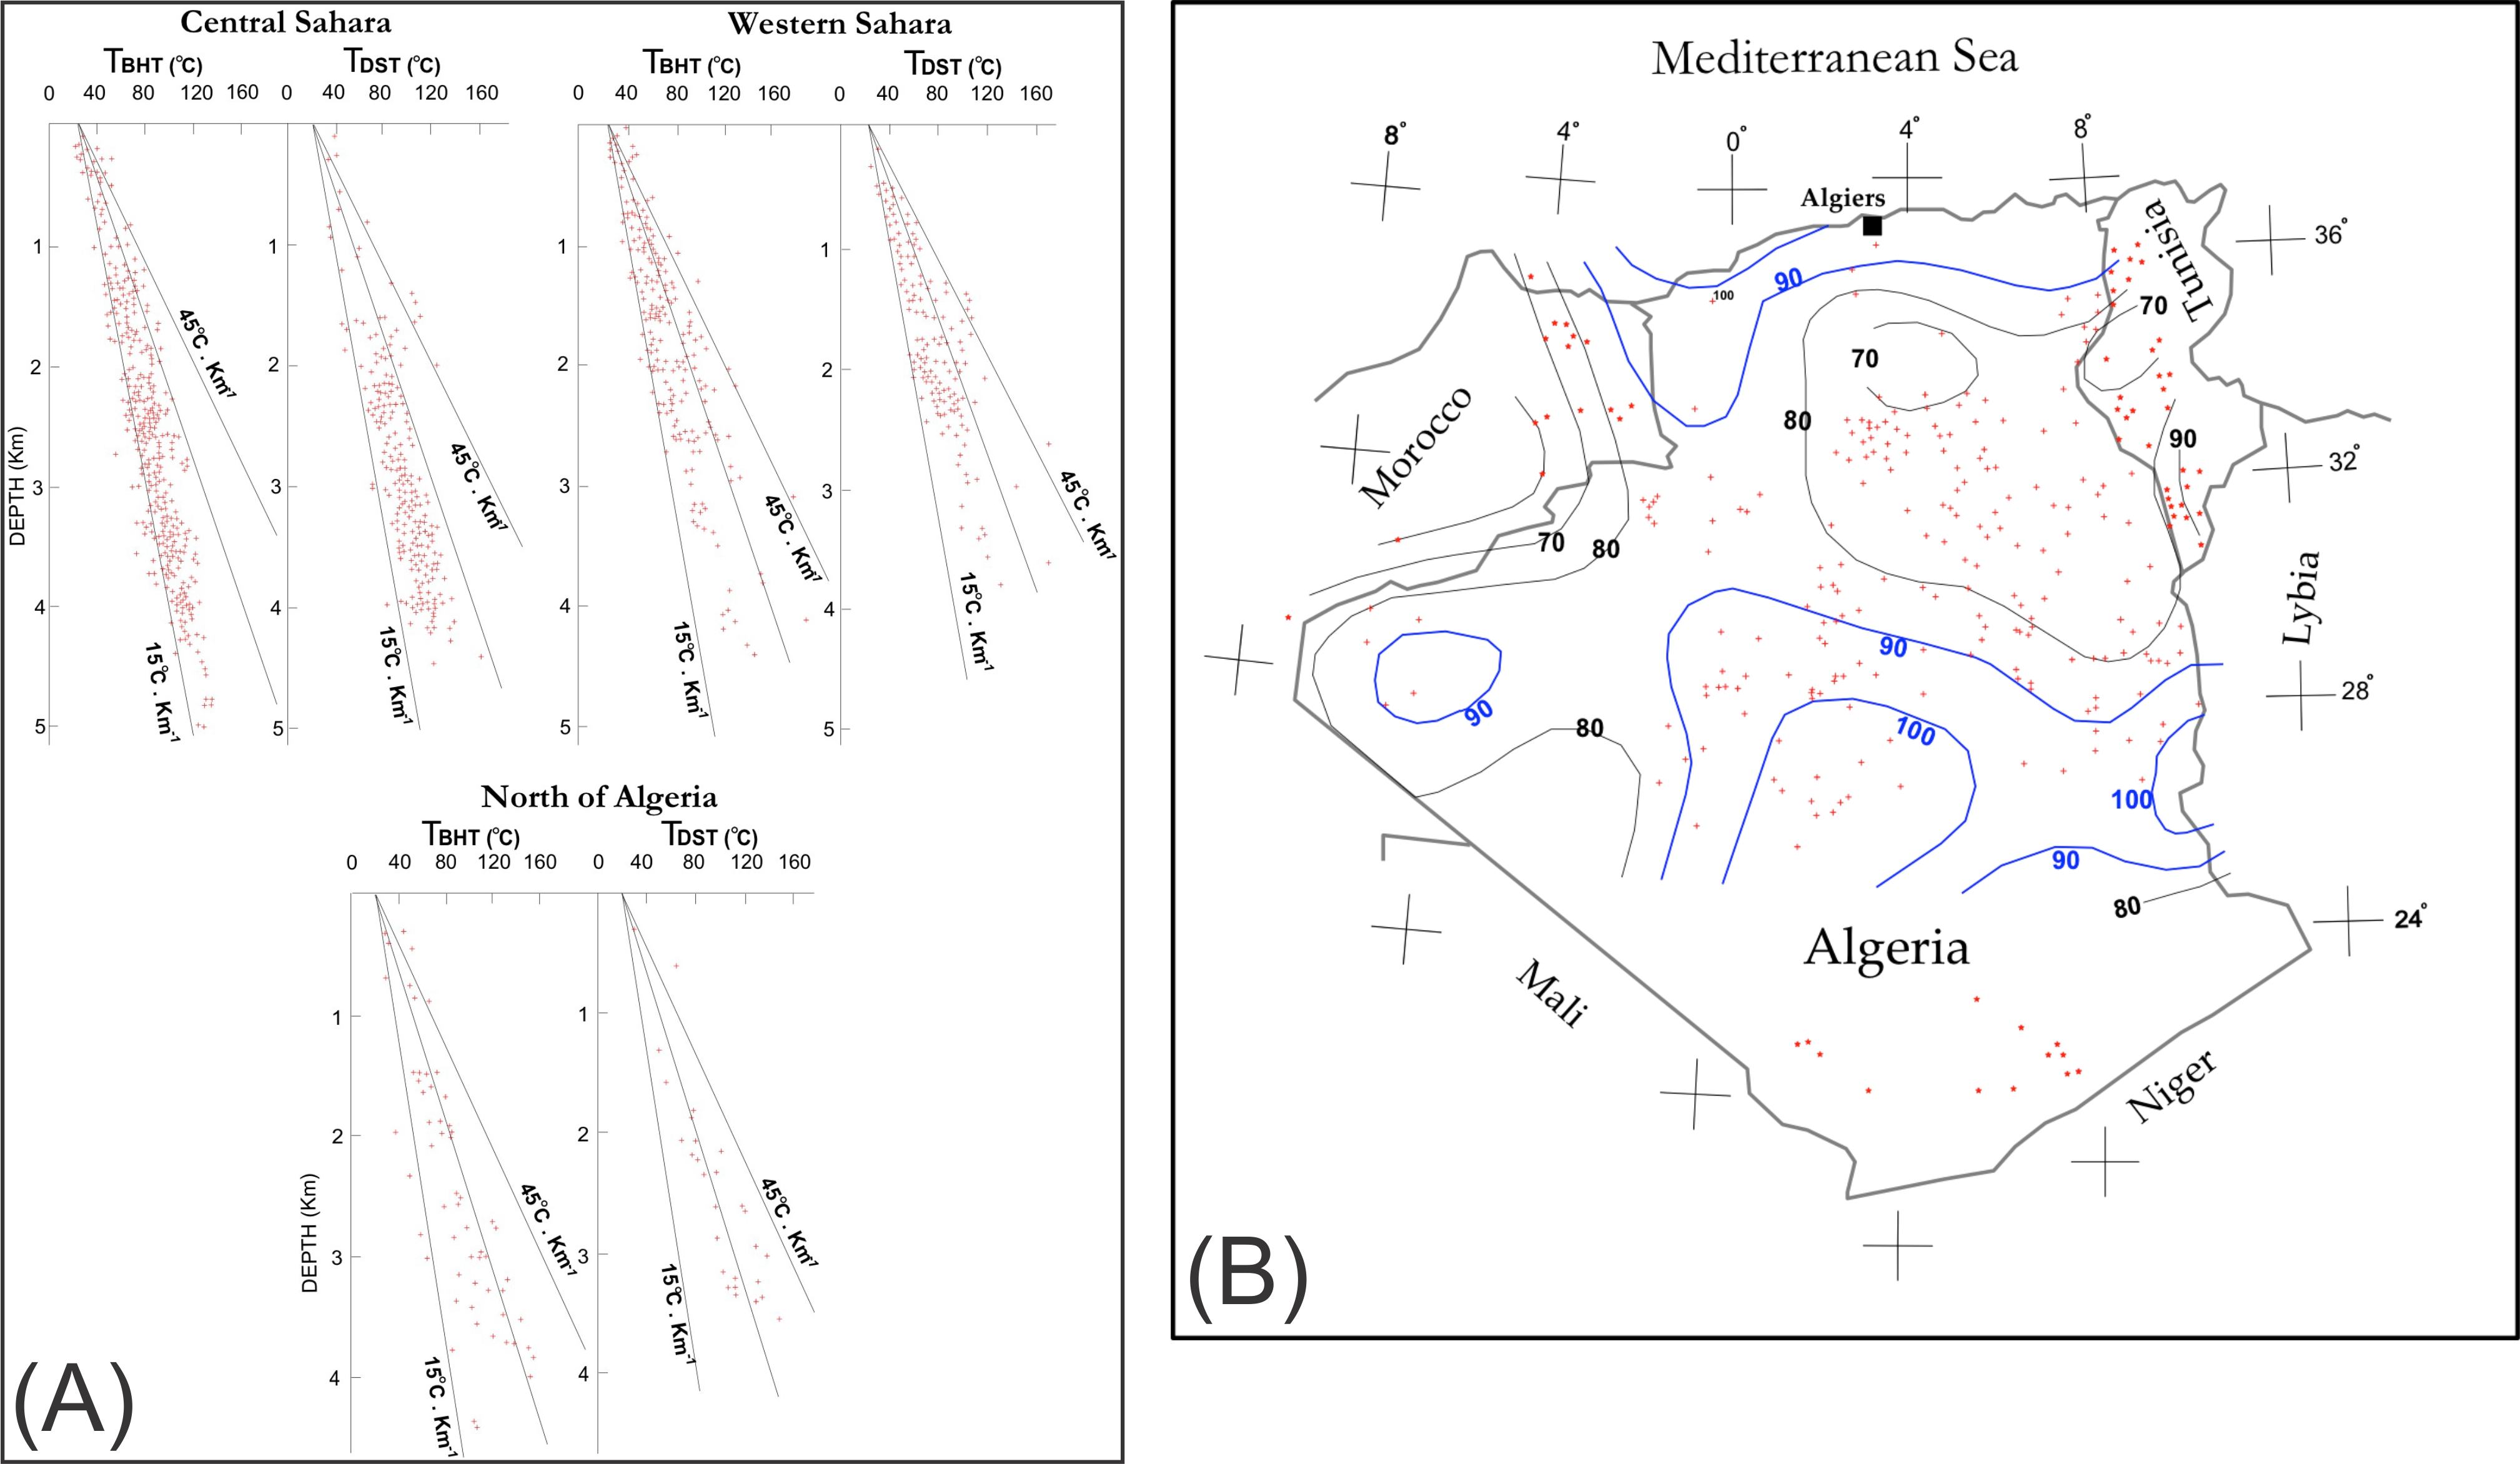
\includegraphics[width=1.0\linewidth]{Fig2}
\captionof{figure}{\color{Green} (A) Temp. vs. depth for different regions (Takherist and Lesquer, 1989). (B) Heat flow map of Algeria (Takherist and Lesquer, 1989). Unit: mW/m$^2$. 230 oil wells are presented, with depths ranging from 500 to 5500 m.}
\end{center}\vspace{1cm}

%------------------------------------------------

\subsection*{Geothermal Reservoirs}
\begin{enumerate}
\item The Tlemcenian dolomites in the NW-Algeria: thermal waters are related to the Plio-Quaternary volcanic rocks; bicarbonate water type.
\item Carbonate formations in the NE-Algeria: area is 15,000 km$^2$; high flow rates (\textgreater100 L/s); highest temperature in Algeria (98 $^{\circ}$C). 
\item Albian sandstone reservoir in the South of Algeria: area is 600,000 km$^2$; depth of aquifer is 2.6 km; highly mineralized waters.
\end{enumerate}
\begin{center}\vspace{1cm}
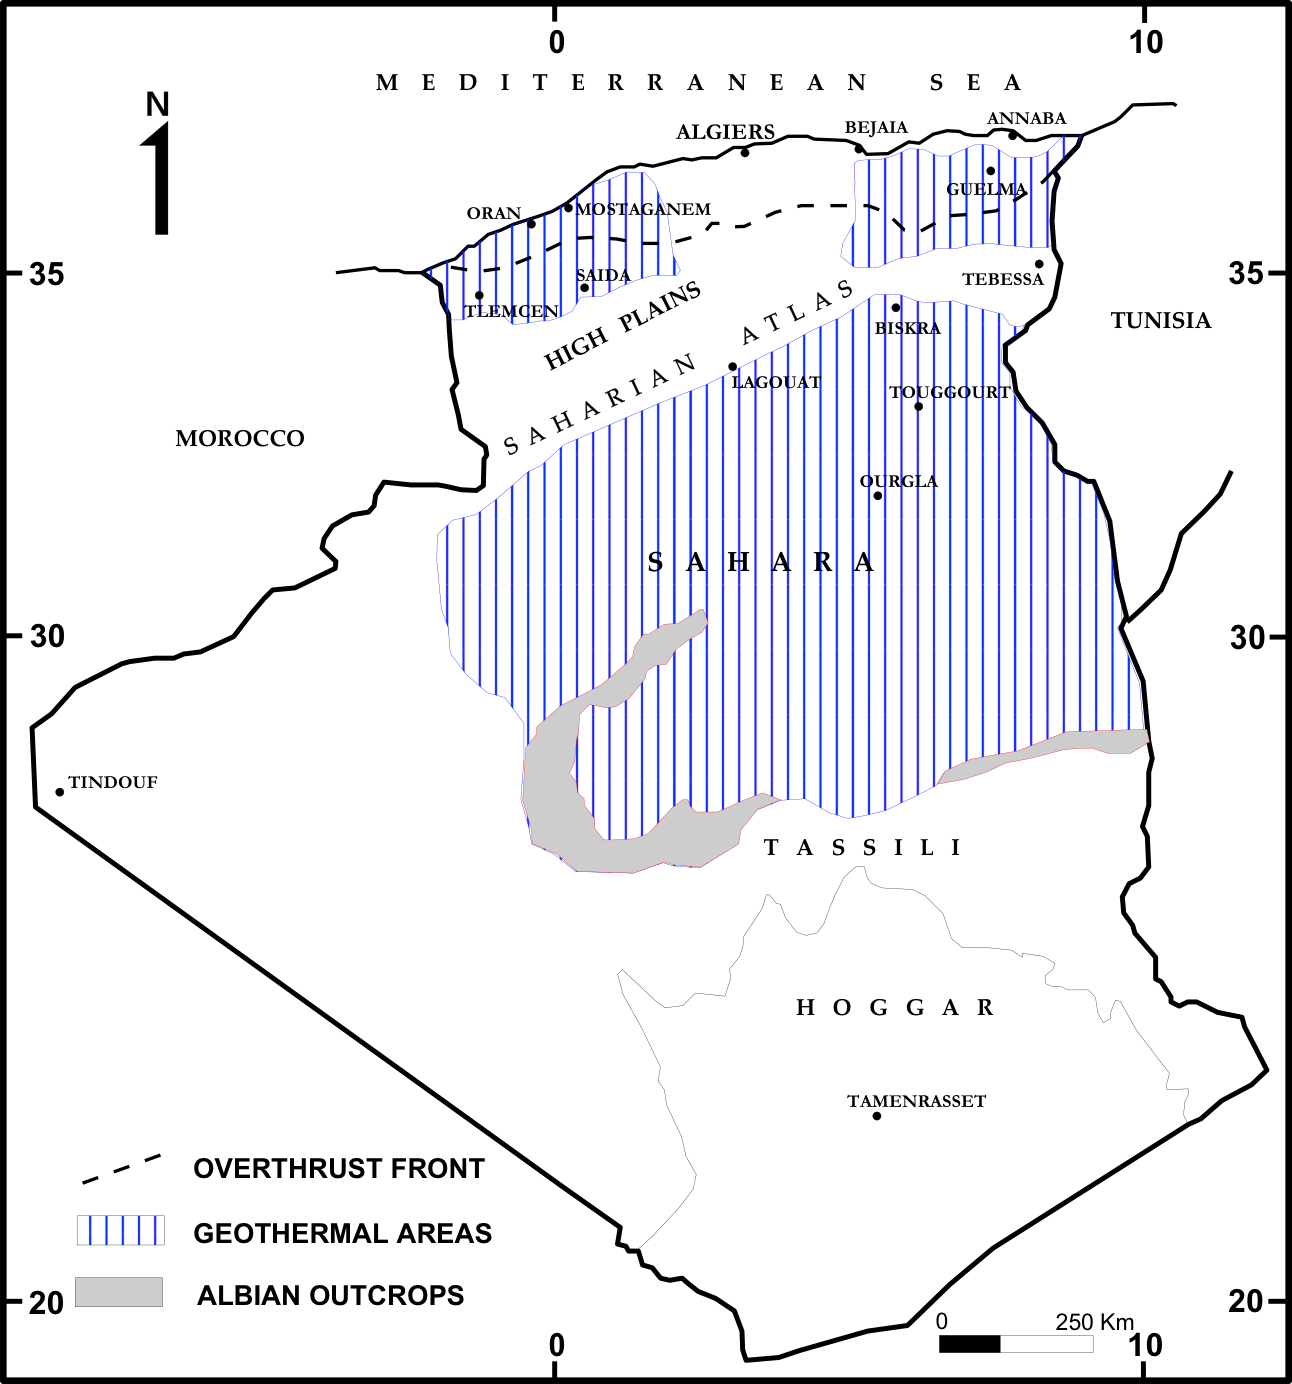
\includegraphics[width=0.8\linewidth]{Figure_4}
\captionof{figure}{\color{Green} Main Algerian geothermal areas (Fekraoui and Abouriche, 1995)}
\end{center}\vspace{1cm}

\subsection*{Hot Springs}
\begin{center}\vspace{1cm}
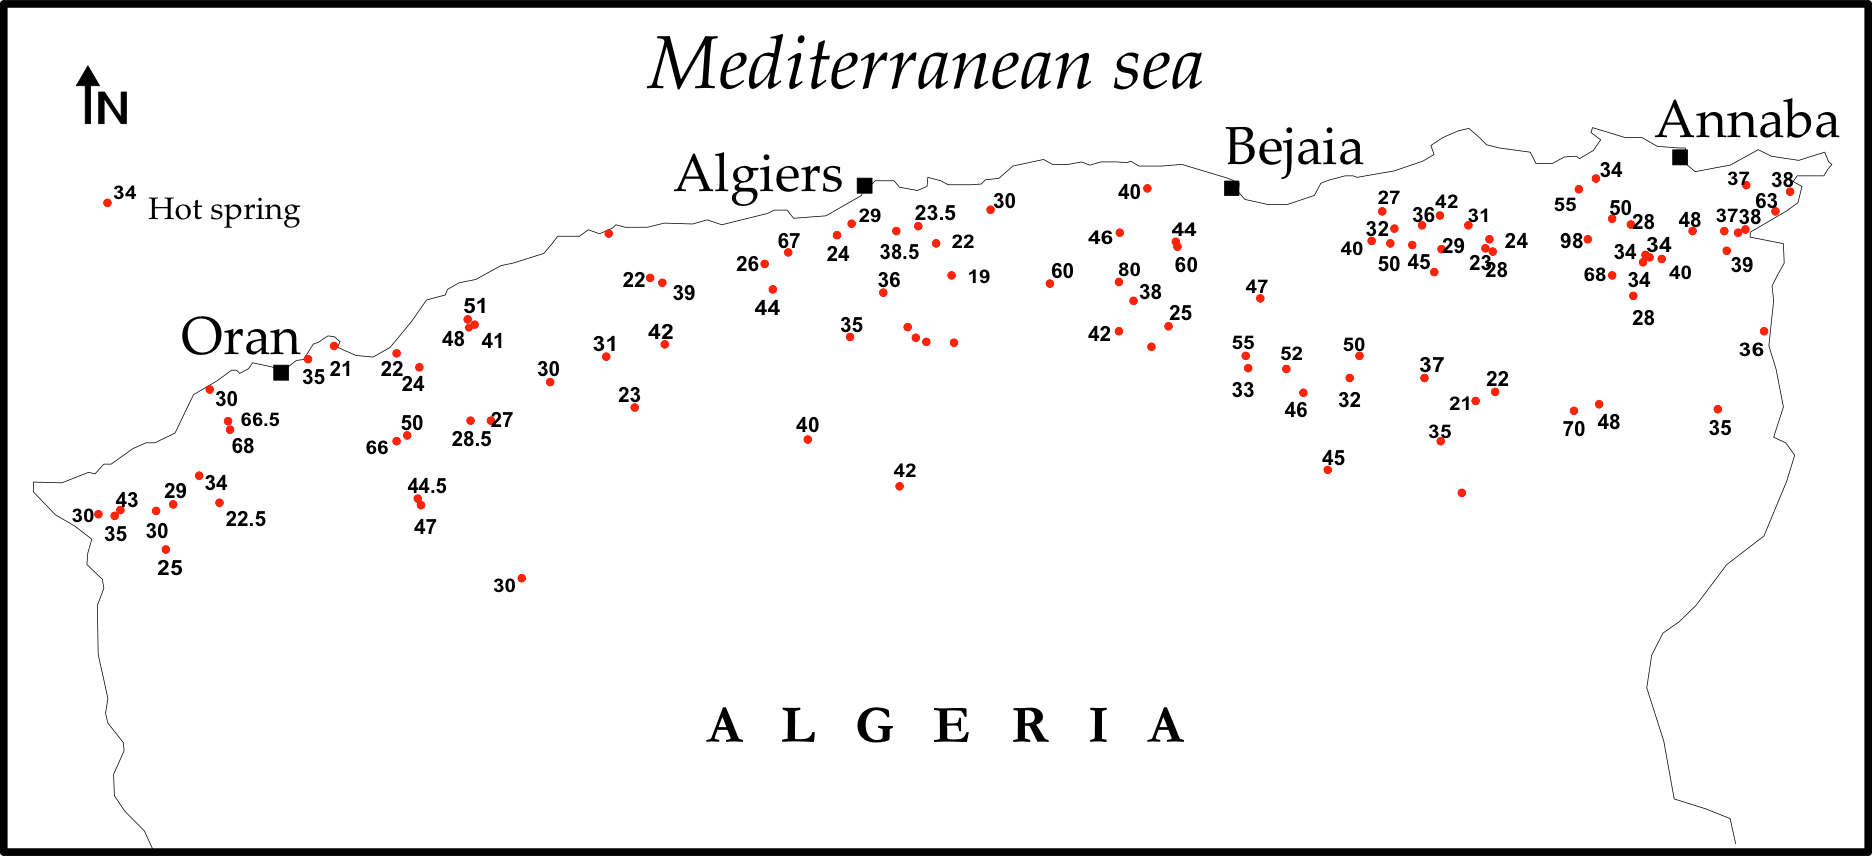
\includegraphics[width=0.8\linewidth]{Figure_5}
\captionof{figure}{\color{Green} Temperatures of the main hot springs of the northern part of Algeria (Kedaid, 2002)}
\end{center}\vspace{1cm}

\begin{center}\vspace{1cm}
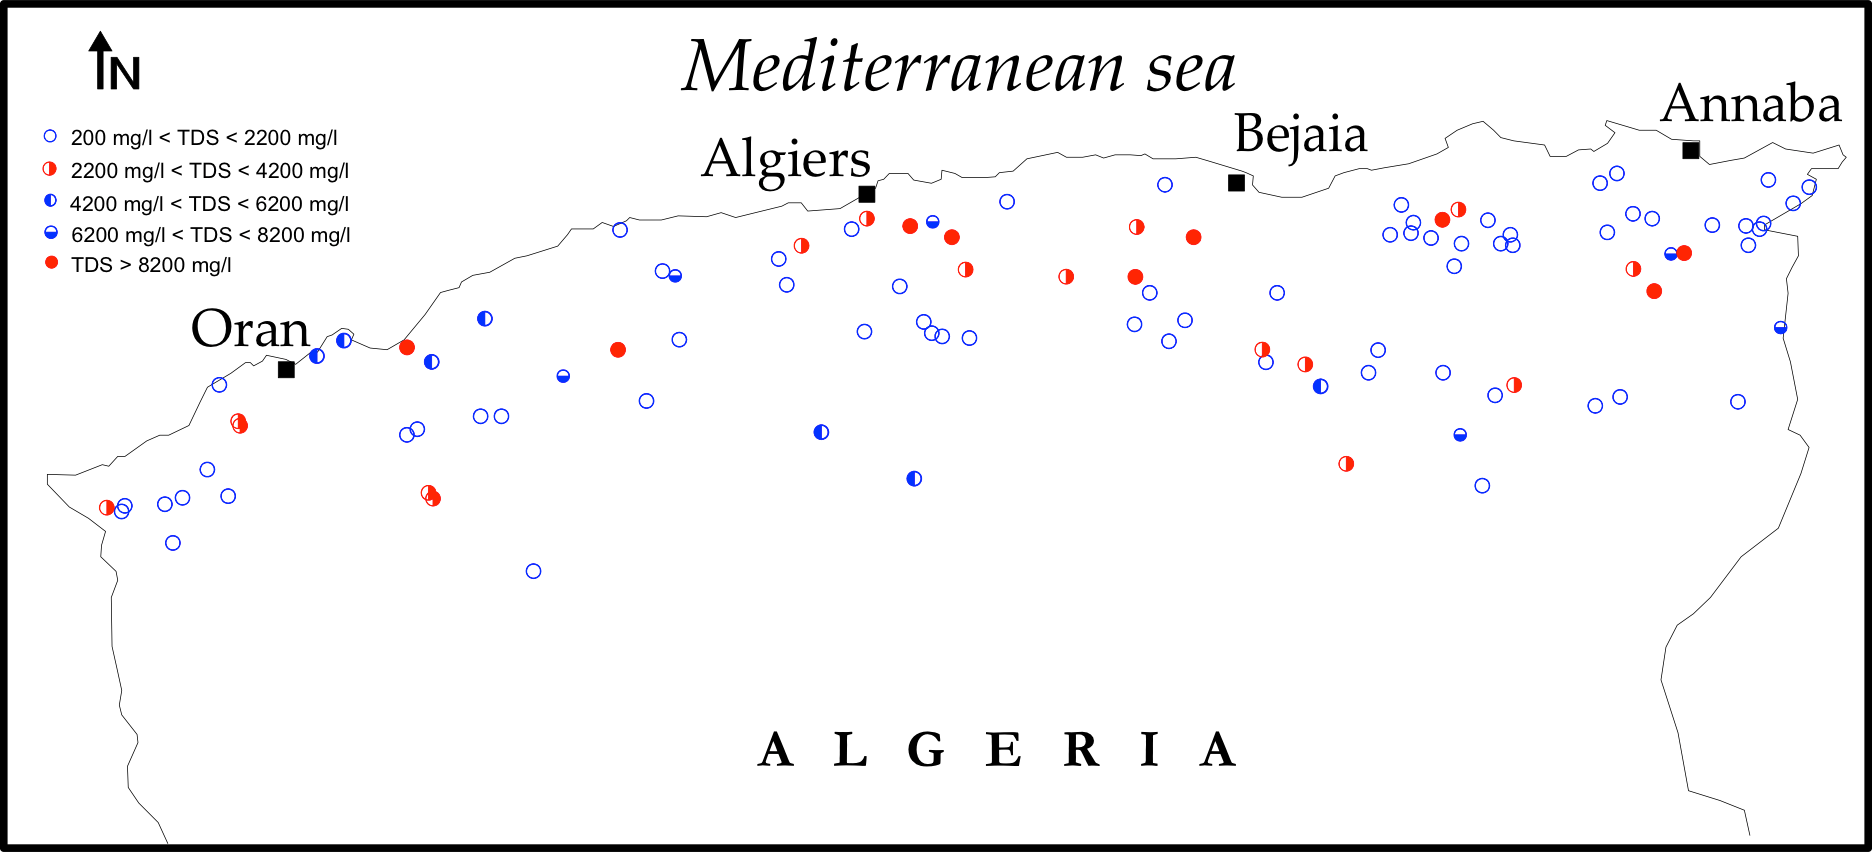
\includegraphics[width=0.8\linewidth]{Figure_6}
\captionof{figure}{\color{Green} Total Dissolved Solid (TDS) of the main hot springs of the northern part of Algeria (Kedaid, 2002)}
\end{center}\vspace{1cm}

\begin{center}\vspace{1cm}
\includegraphics[width=1.0\linewidth]{Fig6.jpg}
\captionof{figure}{\color{Green} (A) Mixing model to illustrate the relative contribution of magmatic, meteoric and crustal sources of gases in NE Algerian geothermal discharges. (B) Photo of the concretions of Hammam Meskhoutine (NE Algeria). The height of the concretions on successive conduits reaches 30 m.}
\end{center}\vspace{1cm}

\subsection*{Geothermal Energy and its uses}
\begin{itemize}
\item Utilizations of the hot water in Algeria are balneology, space and greenhouse heating. 
\item Heat-pump in a primary school (NW Algeria) for heating and cooling purposes.
\item Tilapia fish farming in south of Algeria (Ghardaia and Ouargla).
\item Greenhouses for melon and tomato cultivation in South of Algeria (Ouargla and Touggourt).
\item Future projects: binary-cycle geothermal power plant in Guelma (NE-Algeria); heat-pump in Khenchla (NE Algeria).
\end{itemize}
The total energy use for geothermal is about 1,778.65 TJ/yr.

\begin{center}\vspace{1cm}
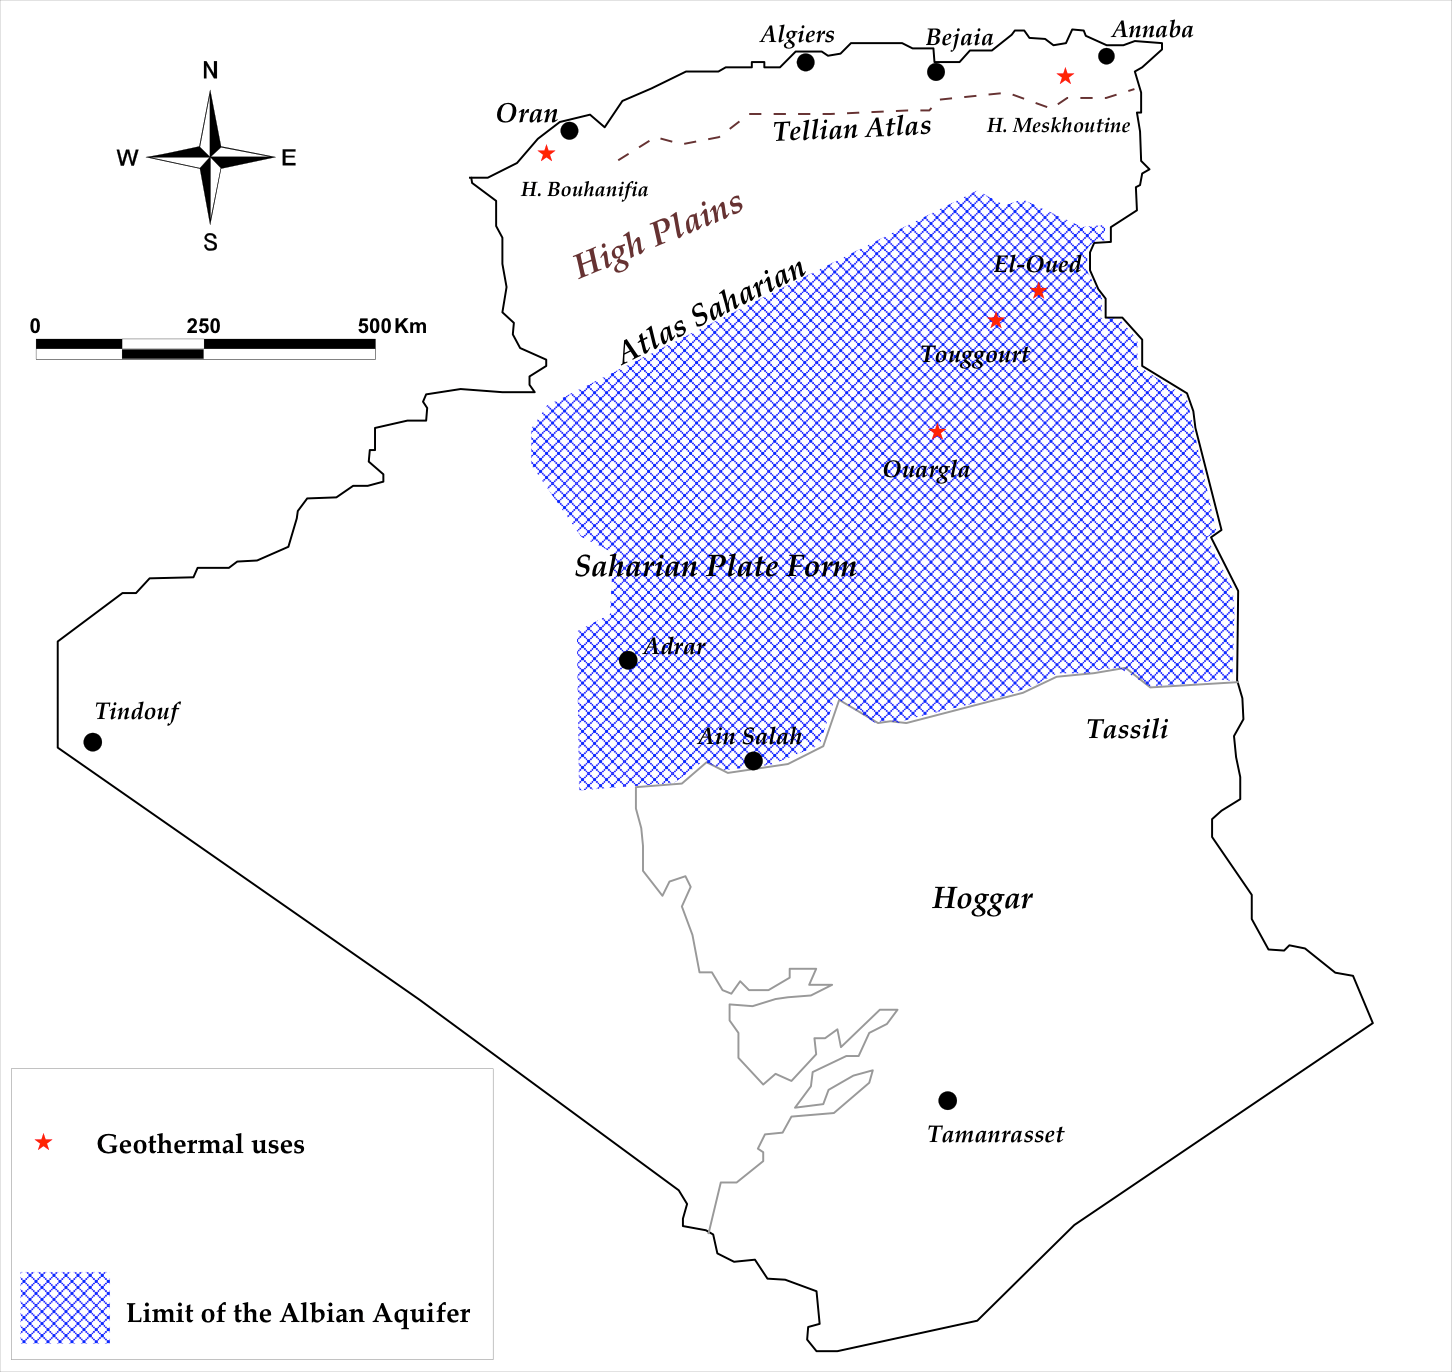
\includegraphics[width=0.8\linewidth]{Figure_7}
\captionof{figure}{\color{Green} Location of Algerian geothermal uses sites (Fekraoui and Kedaid, 2005)}
\end{center}\vspace{1cm}

\subsection*{Geothermal Conceptual Models}
\begin{center}\vspace{1cm}
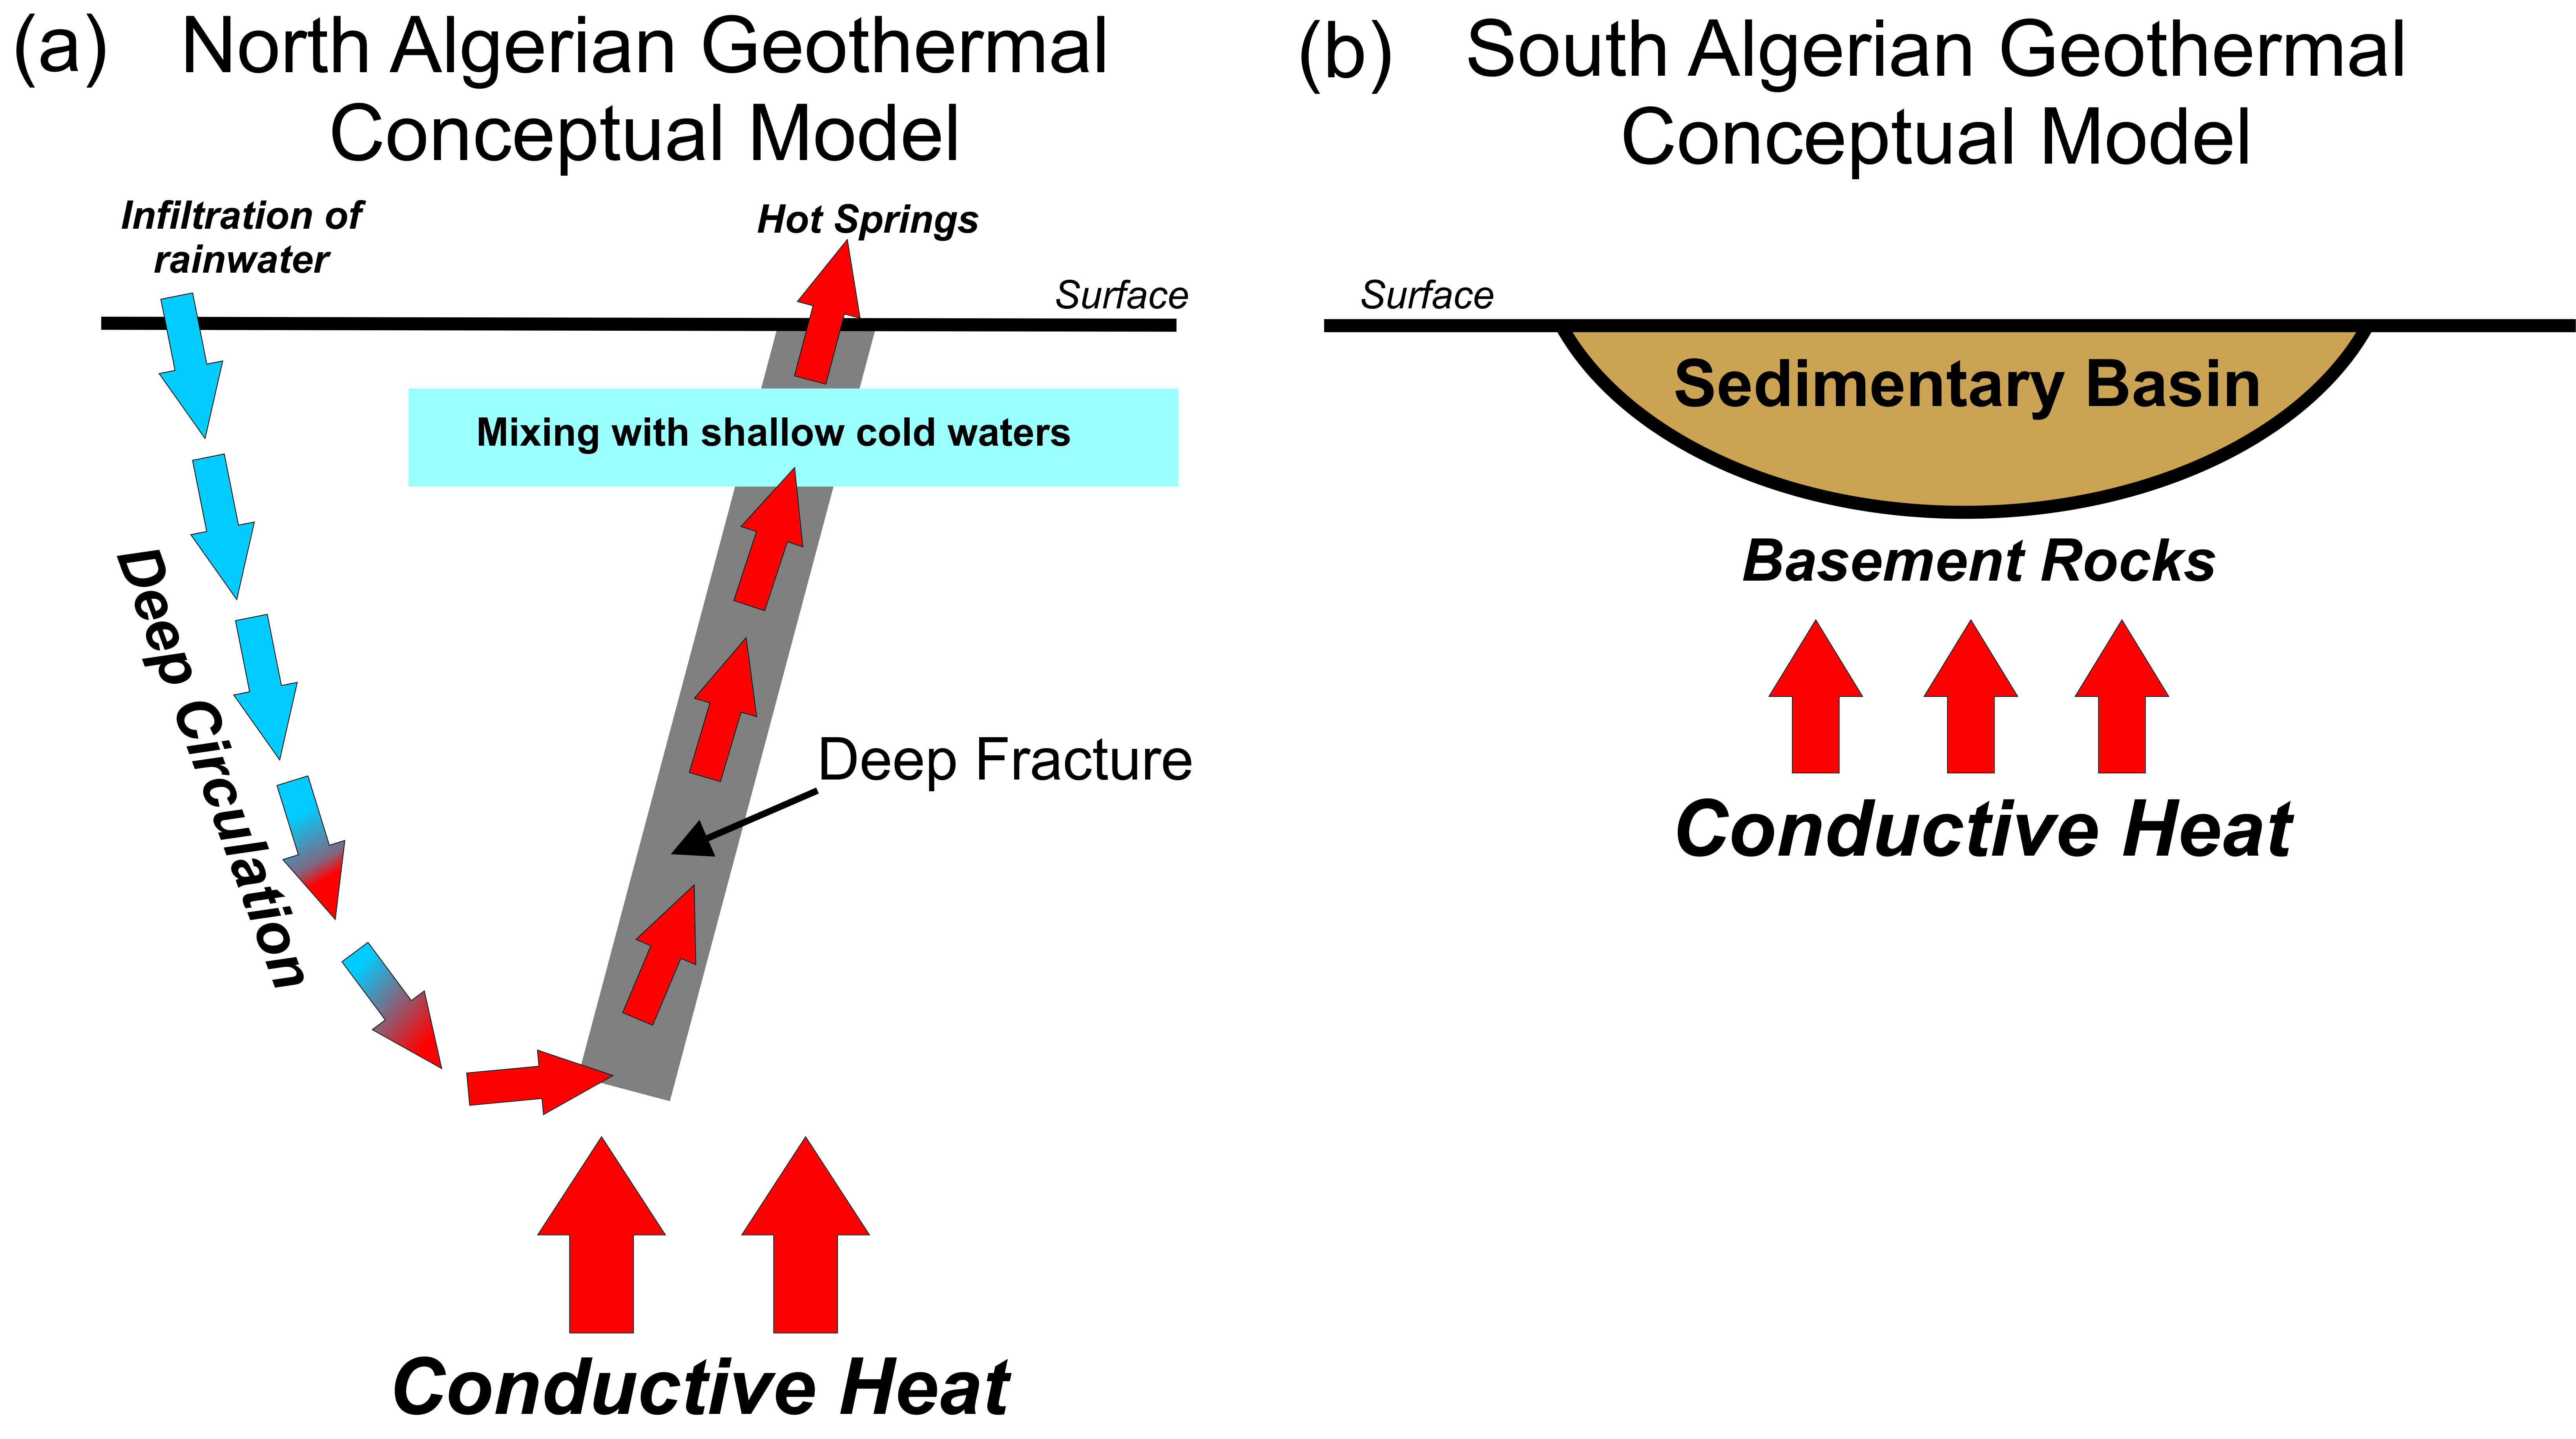
\includegraphics[width=1.0\linewidth]{Algerian_geothermal_models.jpg}
\captionof{figure}{\color{Green} (a) Idealized northern Algerian geothermal system characterized by heating of the filtered meteoric water. (b) Idealized southern Algerian geothermal system, characterized by basement heating of the sedimentary basin (Saibi, 2009)}
\end{center}

%----------------------------------------------------------------------------------------
%	CONCLUSIONS
%----------------------------------------------------------------------------------------

\color{SaddleBrown} % SaddleBrown color for the conclusions to make them stand out

\section*{Conclusions}
Despite being a petroleum- and gas-rich country, Algeria is making efforts to exploit its renewable energies. The Algerian government has adopted new renewable energy laws and financial support for the investors to facilitate the exploitation of the renewable energies for electricity production and direct utilizations. Algeria has relatively abundant geothermal resources especially in the northeastern parts but not totally used.
\color{Black} % Set the color back to DarkSlateGray for the rest of the content

%----------------------------------------------------------------------------------------
%	FORTHCOMING RESEARCH
%----------------------------------------------------------------------------------------

\section*{Forthcoming Research}

Simulation of thermodynamic properties of the thermal fluid and power output with longevity using geological, hydrogeological, and geothermal data from NE-Algerian geothermal reservoirs. 

 %----------------------------------------------------------------------------------------
%	REFERENCES
%----------------------------------------------------------------------------------------

\nocite{*} % Print all references regardless of whether they were cited in the poster or not
\bibliographystyle{plain} % Plain referencing style
\bibliography{sample} % Use the example bibliography file sample.bib

%----------------------------------------------------------------------------------------

\end{multicols}
\end{document}